\documentclass[10pt,a4paper]{article}
\usepackage[T1]{fontenc}
\usepackage[utf8]{inputenc}
\usepackage{lmodern}
\usepackage[margin=23mm]{geometry}
\usepackage{amsmath,amssymb,amsthm,booktabs,tabularx,graphicx,microtype}
\usepackage{enumitem}
\setlist[enumerate]{nosep,leftmargin=1.5em,topsep=3pt}
\usepackage[numbers,sort&compress]{natbib}
\usepackage[font=small,labelfont=bf]{caption}
\usepackage{xcolor}
\usepackage[colorlinks=true,allcolors=blue!45!black]{hyperref}
\setlength{\parskip}{3pt}
\setlength{\textfloatsep}{12pt}
\setlength{\bibsep}{2pt}
\renewcommand{\topfraction}{0.9}
\renewcommand{\bottomfraction}{0.8}
\renewcommand{\textfraction}{0.08}
\renewcommand{\floatpagefraction}{0.8}
\setcounter{topnumber}{3}
\setcounter{totalnumber}{4}
\renewcommand{\bibfont}{\small}
\newtheorem{proposition}{Proposition}
\title{Epiplexity and Transfer in\\Synthetic Time-Series Pretraining}
\author{Danila Chernousov \quad Mark Ikonnikov\\Daniil Kazachkov \quad Alexey Kravatskiy\\[3pt]
\small Moscow Institute of Physics and Technology}
\date{13 November 2026}
\hypersetup{pdftitle={Epiplexity and Transfer in Synthetic Time-Series Pretraining},
pdfauthor={Danila Chernousov, Mark Ikonnikov, Daniil Kazachkov, Alexey Kravatskiy}}
\begin{document}
\maketitle
\begin{abstract}
Can the information acquired during synthetic pretraining help identify useful
data sources for forecasting? We study excess prequential loss, a learning-curve
estimate motivated by epiplexity, across eleven synthetic generators. Models
trained under a common setup are evaluated on real forecasting tasks. The
estimate has a weak association with transfer across the full comparison,
and its value is sensitive to the predictor used as the learning-curve
endpoint. We also explain how prequential and requential coding apply when
training uses losses other than negative log-likelihood. A proper-score
decomposition and a counterexample show why the native training-loss area
requires its own interpretation. Together, the analysis and experiments
clarify the choices needed to measure learned structure and assess its
usefulness for data selection.
\end{abstract}

\section{Introduction}
A synthetic generator can supply an unlimited number of time series, but its
value for pretraining depends on what those series teach a forecasting model.
Periodic signals, stochastic processes, and chaotic dynamics contain different
predictive patterns. A practical question is whether a measurement collected
during training can help choose among them before evaluating every trained
model on real data.

Epiplexity describes structure accessible under a computational
budget~\cite{finzi2026}. It motivates the hypothesis that a source from which
a model acquires more structure will support better transfer. We examine
this hypothesis through excess prequential loss: the accumulated prediction
loss above a held-out final-model loss. The measurement is inexpensive to
collect during probabilistic training.

We analyze completed experiments with eleven generators, one Moirai
architecture, and two training budgets. Across the full set, the measured
area has a weak association with downstream forecasting quality. The
analysis identifies endpoint choice and extreme forecast errors as useful
diagnostics. Our implementation and small application examples are described
in the companion \texttt{episynth} technical report.

We also address a practical measurement question raised by forecasting models
trained with quantile or generative losses. Coding uses probabilities, while
optimization can use another objective. We explain this distinction for both
prequential and requential coding, derive the endpoint correction for a proper
score, and show how two common forecast scores can reverse a ranking. These observations
connect the existing coding constructions to experimental choices.

\section{Background and related work}
\paragraph{Description length and learned structure.}
The minimum description length principle evaluates a model through the cost
of describing it and the remaining cost of describing data given that model.
Prequential coding implements a sequential version: predict a batch, encode
it, then update the predictor. Blier and Ollivier~\cite{blier2018} apply such
codes to neural networks. Finzi et al.~\cite{finzi2026} define epiplexity using
the model-description part of a compute-bounded code and study practical
learning-curve estimates. Qiu et al.~\cite{qiu2026} introduce requential
coding, which reconstructs a student through teacher-generated training samples.

\paragraph{Data selection and forecasting.}
Su et al.~\cite{su2026} use estimated epiplexity gains to guide data selection
and generation for transfer. Synthetic forecasting provides a controlled
setting for testing the same motivation. KernelSynth was introduced with
Chronos~\cite{ansari2024}. Nagpal et al.~\cite{nagpal2026} show that synthetic
generator rankings depend on the forecasting architecture and study mixtures
of generators. We use their generator families with a Moirai
observer~\cite{woo2024} and GIFT-Eval~\cite{aksu2024}. Our question concerns
the relationship between a training-time measurement and subsequent transfer
under this fixed setup.

\paragraph{Forecast losses.}
Proper scoring rules reward a forecast distribution that matches the data
distribution~\cite{gneiting2007}. They connect expected loss to a generalized
entropy and divergence. One example is the continuous ranked probability
score (CRPS), which compares a forecast's cumulative distribution to the
observed outcome. Quantile forecasting models, including
Chronos-2 and TiRex~\cite{ansari2025chronos2,auer2025}, motivate measuring
models trained beyond log-loss. Diffusion objectives also admit variational
interpretations for specified noise weightings~\cite{kingma2023}.
Section~\ref{sec:other} uses these connections to separate the optimization
objective from the quantity accumulated for coding.

\section{Coding measurements}
Let $C$ be the observed past and $Y$ the forecast horizon. A generator defines
a distribution $P(C,Y)$. A predictor $q_i(Y\mid C)$ is evaluated before its
update on the batch containing example $i$. Unless marked as bits, logarithms
are natural and losses are in nats per window. For continuous observations,
log densities give idealized scores. Coding actual observations also requires
a common precision convention and probability masses for the resulting cells.

Formal epiplexity concerns an optimal two-part code under a time budget.
Fix a target dataset of $D$ windows, with contexts $\mathbf C$ and targets
$\mathbf Y$. With shared context and a fixed observation representation, write
\begin{equation}
 q_T^\star\in\arg\min_{q\in\mathcal P_T}
 \bigl\{|q|+\mathbb E[-\log_2 q(\mathbf Y\mid\mathbf C)]\bigr\},
 \qquad S_T(\mathbf Y\mid\mathbf C)=|q_T^\star|,
\end{equation}
where programs in $\mathcal P_T$ evaluate probabilities and sample within
the time bound, and $|q|$ is their description length~\cite{finzi2026}.
For independent windows, the residual cost is $D$ times the predictive risk
in bits. $D$ specifies the dataset whose information is studied. Our
experiments fix an observer and training recipe and measure its trajectory.

\subsection{Prequential loss and its endpoint}
Encoder and decoder start with the same predictor and update rule. Each batch
is encoded under the current predictive distribution. After decoding it,
both sides perform the same update. This gives the idealized data cost
\begin{equation}
 L_{\rm pre}=\sum_{i=1}^N-\log q_i(Y_i\mid C_i).
\end{equation}
The learning-curve estimate subtracts the predictive cost of the final model
on fresh data. If $\widehat R_f$ is its held-out mean loss, the signed area is
\begin{equation}
 A_N=L_{\rm pre}-N\widehat R_f.
 \label{eq:area}
\end{equation}
It summarizes excess loss during the selected training procedure. Its use as
a model-description estimate follows the approximation discussed by Finzi
et al.~\cite{finzi2026}. The total prequential cost has an explicit sequential
coding construction, while the subtraction estimates its structural part.

Endpoint choice enters linearly. Changing the estimated final risk by
$\delta$ changes $A_N$ by $-N\delta$. Our primary endpoint uses an exponential
moving average (EMA) of model weights. Relative to a raw-weight endpoint,
this adds $N(\widehat R_{\rm raw}-\widehat R_{\rm EMA})$. We therefore report
both choices when assessing sensitivity.

\subsection{Requential coding}
Requential coding trains a student on samples from a teacher. Relative entropy
coding communicates these samples using the student's distribution and shared
randomness. The decoder regenerates each sample and repeats the student update,
reconstructing the trained student~\cite{qiu2026}.

Let $Q_k$ and $P_k$ be the teacher and student distributions for a whole
message at step $k$, conditional on the shared history and context. KL
divergence measures the extra expected log-loss from using the student
distribution to predict teacher samples. With
$D_k=\mathrm{KL}_2(Q_k\|P_k)$ in bits, the construction gives
\begin{equation}
 \mathbb E L_{\rm req}\le C_{\rm setup}+
 \sum_k\mathbb E\bigl[D_k+2\log_2(1+D_k)+\kappa\bigr],
 \qquad \kappa<5.21.
 \label{eq:req}
\end{equation}
The expectations include the training trajectory. The cumulative KL is the
leading term, and the remaining terms account for coding overhead. Contexts
and initialization must be shared or included in the setup cost.

A scientific estimate can sample directly from the teacher. Exact
encoder--decoder replay additionally requires a sampling codec and
reproducible updates. Our archived results contain prequential measurements.

\subsection{Training with other losses}\label{sec:other}
The update-rule formulation permits either construction to use a native
non-NLL objective $J$~\cite{qiu2026}. First specify a normalized forecast
distribution, its evaluation convention, observation precision, and shared
contexts. A density head supplies log probabilities directly. A quantile
head needs ordered quantiles, interpolation, tails, and a joint factorization.
A diffusion or flow model needs likelihood evaluation or a specified
latent-variable code. Record any approximation used in evaluating probabilities.

\paragraph{Prequential recipe.}
\begin{enumerate}
\item Generate a fresh batch $(C,Y)$. Before updating, evaluate and save each
window's NLL $-\log q_i(Y\mid C)$ under the coding distribution.
\item Update the model using $J$ on that batch. Keep the native training loss
and coding NLL as separate logs, with the initialization and update settings.
\item After $N$ windows, score the preselected final raw or EMA predictor on
$M$ independent windows from the same generator. Report $L_{\rm pre}$,
$\widehat R_f$, and $A_N=L_{\rm pre}-N\widehat R_f$. Divide by $\ln 2$ for bits.
\end{enumerate}

\paragraph{Requential recipe.}
\begin{enumerate}
\item Train a teacher on generator data using $J$, then freeze a checkpoint
or declare a checkpoint schedule. Initialize a separate student. Specify
teacher and student distributions with finite teacher-to-student KL.
\item At each step, draw targets $\widetilde Y_j$ from the teacher for shared
contexts $C_j$. Before updating the student, save the log ratios. For a
message of $B_k$ conditionally independent windows, use
\begin{equation}
 \widehat D_k=\sum_{j=1}^{B_k}
 \log_2\frac{q_k^{\rm teacher}(\widetilde Y_j\mid C_j)}
 {q_k^{\rm student}(\widetilde Y_j\mid C_j)}.
 \label{eq:req-mc}
\end{equation}
This estimates whole-message KL. Train the student on those sampled targets
using its chosen objective $J$ and a reproducible update rule.
\item Report $\sum_k\widehat D_k$, its sampling uncertainty, message sizes,
the overhead in Eq.~\eqref{eq:req}, and the student's held-out quality.
The measurement describes this student trajectory. A certified code bound
requires controlling the error in the KL estimates.
\end{enumerate}

The native loss also has a useful interpretation. For a loss-oriented proper
score $s$, define its risk $R_s(P,q)=\mathbb E_{Y\sim P}s(q,Y)$,
entropy $H_s(P)=R_s(P,P)$, and divergence
$D_s(P,q)=R_s(P,q)-H_s(P)$. For conditional forecasting, these expressions
include an expectation over $C$. The following identity makes the baseline
choice explicit.

\begin{proposition}[Area relative to a final predictor]
For a fixed distribution $P$, predictors $q_1,\ldots,q_N$, and a final
predictor $q_f$, suppose the score risks are finite. Then
\begin{equation}
 \sum_{i=1}^N\{R_s(P,q_i)-R_s(P,q_f)\}
 =\sum_{i=1}^N D_s(P,q_i)-ND_s(P,q_f).
 \label{eq:proper}
\end{equation}
\end{proposition}
\begin{proof}
Substitute $R_s(P,q)=H_s(P)+D_s(P,q)$ in each term. The entropy terms cancel.
\end{proof}
For random training trajectories the identity holds after taking expectation.
Fresh training examples and an independent held-out endpoint estimate connect
it to the expected measured area. Referencing the Bayes risk $H_s(P)$ instead
gives accumulated divergence directly. Log-loss yields KL. CRPS yields
$\int(F_P-F_q)^2\,dy$~\cite{gneiting2007}.

These divergences can order predictors differently. Take
$P=\mathrm{Bernoulli}(0.1)$ and the two predictions in
Table~\ref{tab:counterexample}. For Bernoulli probabilities $p,q$, the
divergences are $(p-q)^2$ and
$p\log(p/q)+(1-p)\log((1-p)/(1-q))$, respectively.
CRPS favors the prediction near zero, whereas
KL strongly penalizes its low probability for the outcome one. Repeating
either predictor for the same number of steps and finishing at $q_f=P$
gives reversed area rankings. Thus a common ranking requires additional
assumptions on the distributions or learning trajectories.

\begin{table}[htbp]
\centering\small
\caption{Ranking reversal for a fixed Bernoulli truth with success probability
0.1. Lower divergence is better. Values are computed directly.}
\label{tab:counterexample}
\begin{tabular}{@{}rrr@{}}
\toprule
Predicted success probability & CRPS divergence & KL (nats)\\
\midrule
0.3 & 0.040000 & 0.116322 \\
0.001 & 0.009801 & 0.366593 \\
\bottomrule
\end{tabular}

\end{table}

For diffusion, a complete negative evidence lower bound (ELBO) on the same
observations can be written as
$B_i=R_{\log}(P,q_i)+G_i$, where $G_i\ge0$ is the expected variational gap.
With the same endpoint subtraction,
\begin{equation}
 A_{\rm ELBO}=A_{\log}+\sum_iG_i-NG_f.
\end{equation}
The gap's evolution therefore matters to the area. Kingma and
Gao~\cite{kingma2023} relate specified noise weightings to ELBO objectives.
Using such an objective for measurement requires stating its latent variables,
weighting, and data representation. The raw training loss, a likelihood
estimate, and a variational code bound each define a measurable quantity.

\subsection{Choosing synthetic sample sizes}\label{sec:sample-size}
Training length determines how much structure the chosen learner can acquire.
We therefore recommend reporting a curve over training budgets. Keep the
target size $D$ and compute bound $T$ fixed when comparing formal two-part
codes. For the trajectory measurements here, state the training size $N$,
architecture, batch size, and recipe for every comparison.

\paragraph{Training windows.}
Generate fresh windows on demand with disjoint training, validation, and
final-evaluation seed ranges. Count independent generated series as the
sampling units. If several windows come from one series, keep the series
within one split and account for their dependence in uncertainty estimates.
Choose $N$ from the available training compute and measured cost per update.
Use a common grid such as $N,2N,4N$ across sources, fixing the batch size and
declaring the learning-rate schedule. At each budget, inspect validation
quality and the stability of source rankings across independent training
seeds. Increase the common budget while the changes matter for the intended
comparison. For our Moirai setup, the existing 2M-window runs provide a
starting scale, with 40M as a larger-budget sensitivity check.

\paragraph{Evaluation windows.}
Size the final evaluation set from a pilot estimate of per-window NLL
standard deviation $s_f$. For a fixed trained model and $M$ independent
evaluation windows, the endpoint contribution to the area standard error is
\begin{equation}
 \mathrm{SE}_{\rm endpoint}(A_N)\simeq\frac{Ns_f}{\sqrt M},
 \qquad
 M\gtrsim\left(\frac{1.96Ns_f}{\Delta_A}\right)^2.
 \label{eq:sample-size}
\end{equation}
Here $\Delta_A$ is a desired approximate 95\% half-width in nats. This follows
from $A_N=L_{\rm pre}-N\widehat R_f$ and the standard error of a mean, assuming
finite variance and an adequate normal approximation. A practical starting
pilot is $10^4$ independent evaluation windows. Use its variance to set a
fresh final sample size before scoring. Our archived runs used $10^5$
held-out windows per checkpoint. For fixed $\Delta_A$ and variance, doubling
$N$ requires four times as many evaluation windows. Training-seed variation
and likelihood-approximation error require separate assessment.

\paragraph{Teacher and student budgets.}
For requential measurement, record generator windows used to fit the teacher
and teacher-generated targets used to fit the student separately. The
generator also supplies contexts for student training. Start from a fixed
teacher checkpoint and a student-budget grid. Select the first checkpoint
whose validation NLL is within a prespecified tolerance of the teacher's,
then score it on fresh evaluation data. Report each student's budget and
quality gap, including cases that exhaust the budget before reaching the
tolerance. Further training can keep adding KL, so choose the endpoint by
budget and predictive quality.

Extra teacher draws allow an independent audit of a saved teacher/student
pair. If $s_r$ is the pilot standard deviation of the whole-message log
ratio in bits, choose $m\gtrsim(1.96s_r/\delta_D)^2$ independent teacher
messages for an approximate 95\% KL half-width $\delta_D$, under the same
variance assumptions. Keep these audit draws separate from student updates
and record their count. This controls precision for the audited pair.
Use independent training repeats to assess variation in the cumulative
measurement.

\section{Experimental setup}
We use the completed runs archived with \texttt{episynth}~\cite{chernousovresults}.
The eleven generators cover Gaussian-process kernels (KernelSynth), exponential
smoothing (ETS), periodic waveforms, switching stochastic differential equations
(SDE), steps, trend--seasonality--irregularity compositions (TSI), ARIMA,
fractional Brownian motion (fBm), GARCH volatility, chaotic dynamics, and
TimeSynth signals. Each source is studied separately.

The observer is a Moirai port trained from scratch, with six transformer layers,
width 384, patch size 32, and 10,746,600 parameters. Its density head mixes
Student-$t$, fixed-scale Gaussian, and log-normal components. It predicts the
horizon as a product of pointwise densities conditional on context. Context
lengths are sampled from a saved distribution spanning 13 to 512 points.
The target horizon is 64 points. Scaling uses context only, and a small
uniform dequantization smooths observations.

There are approximately 2 million and 40 million windows per primary run.
Both budgets use the same architecture and initialization seed, with one
additional Waveform initialization at the larger budget. The two budgets
share training seed ranges. Within each series, the training-window budget
and optimizer settings are matched. Appendix~\ref{sec:protocol} gives the
exact settings and artifact locations.

Each batch's mean NLL per target point, $u_k$, is recorded before its update.
For batch size $B$, horizon $h$, and $N=BK$ windows, the measured area is
$A_N=Bh\sum_{k=1}^K u_k-N\widehat R_f$. The endpoint is scored on fresh windows
from the same generator. We use every exported batch mean and retain the
signed result in million nats.

Final EMA models are evaluated without fine-tuning on 55 short-term GIFT-Eval
configurations. The main metric is the continuous ranked probability score
(CRPS), which evaluates the predictive distribution. We normalize each
configuration by its seasonal-naive baseline and take an equally weighted
geometric mean:
\begin{equation}
 R_g=\exp\left\{\frac1{55}\sum_{j=1}^{55}
 \log\frac{\mathrm{CRPS}_{g,j}}{\mathrm{CRPS}_{\rm naive,j}}\right\}.
\end{equation}
Smaller values indicate better forecasts, and values below one beat the
baseline. We also examine mean absolute scaled error (MASE), median ratios,
configuration ranks, and mean downstream NLL. The CRPS calculation uses the
saved sample-based score. The separate quantile-loss field is retained as
an additional metric in the data tables.

Spearman correlation compares generator rankings. Its 95\% percentile
intervals use 10,000 paired bootstrap resamples of the eleven families.
These intervals describe variation across sources. Training-seed uncertainty
is assessed only by the additional Waveform run. Related benchmark
configurations are kept together within each generator's aggregate score.

\section{Results}
\subsection{Transfer across synthetic sources}
Under the common training setup, KernelSynth and ETS give the strongest
aggregate transfer at both budgets (Table~\ref{tab:results}). Increasing the
budget improves CRPS for most generators. The improvement is particularly
large for StepFunction, while Waveform and Chaotic remain sensitive cases.
These differences show why source choice matters even with a fixed observer.

\begin{table}[htbp]
\centering\small
\caption{Excess area $A$ in million nats and forecast-error ratios to seasonal
naive. Lower CRPS and MASE ratios are better. Primary runs use seed 0.}
\label{tab:results}
% Generated by analyze_runs.py; values come from run_statistics.csv.
\begin{tabular}{@{}lrrrrrr@{}}
\toprule
 & \multicolumn{3}{c}{2 million windows} & \multicolumn{3}{c}{40 million windows}\\
\cmidrule(lr){2-4}\cmidrule(l){5-7}
Generator & $A_N$ & CRPS & MASE & $A_N$ & CRPS & MASE\\
\midrule
KernelSynth & 68.4 & \textbf{0.678} & \textbf{0.895} & 926.1 & \textbf{0.639} & \textbf{0.828} \\
ETS & 26.7 & 0.731 & 0.963 & 138.6 & 0.717 & 0.941 \\
Waveform & 70.9 & 0.818 & 1.043 & 1061.2 & 1.373 & 0.986 \\
SDE & 11.0 & 0.872 & 1.160 & 34.6 & 0.861 & 1.142 \\
StepFunction & 49.5 & 1.607 & 1.100 & 588.3 & 0.839 & 1.092 \\
TSI & 64.8 & 0.803 & 1.069 & 765.9 & 0.776 & 1.028 \\
ARIMA & 24.2 & 0.847 & 1.108 & 154.5 & 0.833 & 1.089 \\
fBm & 9.6 & 0.853 & 1.094 & 40.6 & 0.867 & 1.110 \\
GARCH & 16.6 & 0.879 & 1.121 & 100.9 & 0.874 & 1.116 \\
Chaotic & 126.2 & 1.171 & 1.478 & 1956.6 & 1.285 & 1.616 \\
TimeSynth & 15.3 & 0.974 & 1.297 & 114.9 & 0.851 & 1.123 \\
\midrule
Waveform, seed 1 & --- & --- & --- & 1063.6 & 0.972 & 0.995 \\
\bottomrule
\end{tabular}

\end{table}

\subsection{Association with the learning-curve area}
Across all eleven generators, the association between area and transfer is
weak at both budgets (Figure~\ref{fig:transfer}, Table~\ref{tab:correlations}).
A negative correlation would support the proposed use of larger area to
identify lower forecasting error. The observed full-set estimates are near
zero, with wide intervals. Final held-out loss also has a weak association.
The current comparison gives little support for choosing a source using
either measurement alone.

\begin{figure}[htbp]
\centering
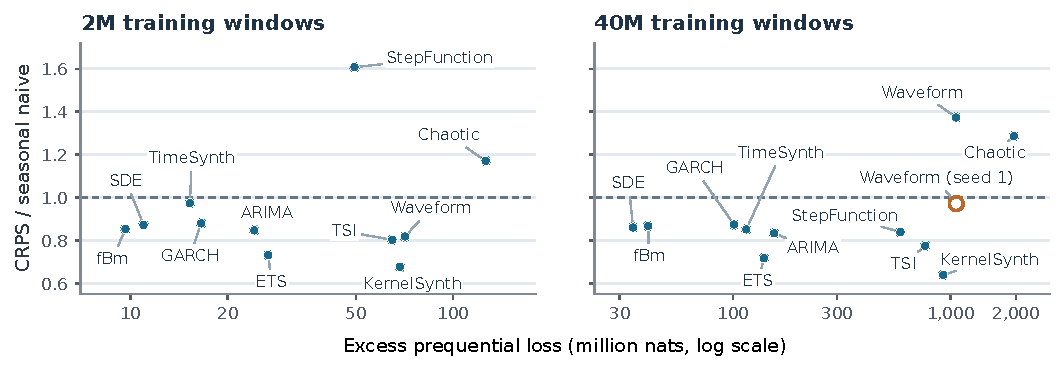
\includegraphics[width=\linewidth]{figures/transfer_results.pdf}
\caption{Excess area and downstream CRPS for all eleven generators.
Labels identify cases discussed in the text. The open point is the additional
Waveform initialization. Dashed lines mark seasonal-naive performance.}
\label{fig:transfer}
\end{figure}

Removing Chaotic and Waveform yields a stronger negative association,
especially at the larger budget. This subset was chosen after examining the
results. Other exclusions and area variants were explored in the archived
analysis, so the subset finding motivates a follow-up on new sources.
Downstream NLL shows a weaker relationship on the same subset.

\begin{table}[htbp]
\centering\small
\caption{Spearman association with downstream CRPS. Intervals resample
generator families. The nine-source subset excludes Chaotic and Waveform
and was selected after inspecting the results.}
\label{tab:correlations}
\begin{tabular}{@{}llrrrr@{}}
\toprule
Budget & Predictor / sources & $n$ & $\rho$ & Lower 95\% & Upper 95\%\\
\midrule
2M & EMA area, all sources & 11 & -0.18 & -0.81 & 0.51 \\
2M & Raw area, all sources & 11 & -0.15 & -0.75 & 0.53 \\
2M & Final loss, all sources & 11 & -0.13 & -0.70 & 0.46 \\
2M & EMA area, selected subset & 9 & -0.47 & -0.95 & 0.39 \\
\midrule
40M & EMA area, all sources & 11 & 0.00 & -0.89 & 0.61 \\
40M & Raw area, all sources & 11 & 0.19 & -0.65 & 0.71 \\
40M & Final loss, all sources & 11 & -0.22 & -0.83 & 0.49 \\
40M & EMA area, selected subset & 9 & -0.82 & -1.00 & -0.28 \\
\bottomrule
\end{tabular}

\end{table}

\subsection{Endpoint and forecast sensitivity}
The EMA endpoint changes the area by the accumulated benefit of averaging
the final weights. ARIMA illustrates the size of this effect: its area at
the larger budget changes by roughly a factor of ten between the raw and
EMA endpoints. Across sources, using the raw endpoint still gives a weak
association with transfer. This supports reporting endpoint sensitivity as
part of the measurement.

Waveform's second initialization has almost the same area as the first,
but substantially better aggregate CRPS. Their median configuration scores
are much closer. The saved summaries locate an extreme error on the
\texttt{bitbrains\_rnd} configuration, showing how a small number of forecast
failures can affect an aggregate. Individual forecast samples would be needed
to identify their cause. Replacing the primary Waveform run with the repeat
leaves the full-set area correlation near zero.

\subsection{Early measurements and a compression baseline}
Seven held-out checkpoints allow area to be recomputed at short prefixes,
using each checkpoint's own endpoint. Their correlations with final transfer
vary with budget and training stage. Checkpoint loss and loss reduction show
similar sensitivity. The accompanying prefix figure and CSV tables preserve
these exploratory comparisons.

A gzip baseline compresses series from ten generators at a common numeric
representation. Its association with CRPS is negative at both budgets, with
intervals spanning zero. This inexpensive baseline remains relevant for a
larger study of source selection. The present uncertainty supports evaluating
candidate signals on additional generators and initialization repeats.

\section{Discussion}
The completed experiments establish a specific empirical result: excess
prequential loss has a weak full-set relationship with transfer under this
Moirai training setup. The best synthetic sources remain useful practical
findings within that setup. Generalization to other architectures, source
mixtures, or training recipes requires new comparisons.

The coding analysis helps define those comparisons. Non-NLL training can be
paired with prequential probability evaluation, provided the predictive
distribution is specified. Requential coding offers a separate route through
student reconstruction and requires an additional training trajectory.
For quantile models, the distribution reconstructed from quantiles becomes
part of the measurement protocol. For diffusion models, likelihood or
variational coding choices determine the reported quantity.

A focused next experiment would compare the prequential area with cumulative
requential KL for a small set of teachers at matched predictive quality.
An OU prior supplies a known Bayesian reference for checking the likelihood
calculation. Repeated initializations would then help separate estimator
sensitivity from variation in learned forecasts. These measurements would
test whether the current relationship depends on the area approximation.

\appendix
\section{Protocol and reproducibility}\label{sec:protocol}
The archived runs were conducted by Danila Chernousov and uploaded at commit
\texttt{7d2b001}. This article recomputes their analysis from committed
configurations, training curves, held-out scores, and benchmark summaries.
There are 22 primary runs and one initialization repeat.

\begin{table}[htbp]
\centering\small
\caption{Settings shared within each budget comparison.}
\begin{tabular}{@{}lrr@{}}
\toprule
Setting & Smaller budget & Larger budget\\
\midrule
Training windows & 1,999,872 & 39,999,488\\
Optimizer steps & 1,953 & 39,062\\
Batch size & 1,024 & 1,024\\
Held-out windows per checkpoint & 100,000 & 100,000\\
\bottomrule
\end{tabular}
\end{table}

Training uses AdamW with learning rate $10^{-3}$, 200 warmup steps, weight
decay 0.1, $\beta=(0.9,0.98)$, $\epsilon=10^{-6}$, and gradient clipping at 1.
The EMA time constant is 2\% of the total step budget. Training uses bfloat16.
Raw and EMA checkpoints are evaluated at 1, 2, 5, 10, 20, 50, and 100\% of
the budget. The primary area uses the matching bfloat16 endpoint. The
Gaussian mixture component has fixed scale $10^{-3}$. Dequantization width
is $10^{-3}\sqrt{\widehat{\mathrm{Var}}(C)+10^{-5}}$.

The shorter series uses precomputed corpora. The longer series generates
windows online except for KernelSynth. Hardware and generation costs vary,
so the comparison matches windows and architecture. Downstream NLL is the
arithmetic mean of original-unit NLL per point across configurations and
retains the evaluator's exclusion of windows with zero seasonal error.

Batch means reconstruct the signed linear area. The six-significant-digit
exports imply a worst-case rounding error below 0.013 million nats. All
primary areas agree with the archived per-window analysis at its displayed
precision. Held-out standard errors require the large per-window files
distributed separately with the experiment artifacts.

From \texttt{publications/article/}, run \texttt{python reproduce.py} to
recompute statistics and figures, then \texttt{python build\_report.py} to
compile this document. The analysis reads the two dated series directories
under \path{experiments/episynth/}. It records input hashes and verification
results in \path{data/analysis_verification.json}. Additional tables contain
per-configuration scores, prefix measurements, and all explored correlations.
The accompanying \texttt{README.md} describes the artifacts and commands.

\bibliographystyle{plainnat}
\bibliography{references}
\end{document}
